\chapter*{MTHE 393 Project Intro}\label{chap:Preface_393}


\tikzstyle{startstop}=[rectangle,rounded  corners, minimum width = 4cm, minimum height = 1cm, text centered, draw=black,  fill  = white]
\tikzstyle{arrow1} = [thick,<->,>=stealth]
\tikzstyle{arrow2} = [thick,->,>=stealth]


MTHE 393 consists of two components: a lab component, and a project component. It is the goal 
of the first four labs in this manual to teach you the skills and concepts necessary to successfully 
complete your project. 

\begin{tabular}{p{4cm} p{10cm}}
\vspace{0pt}

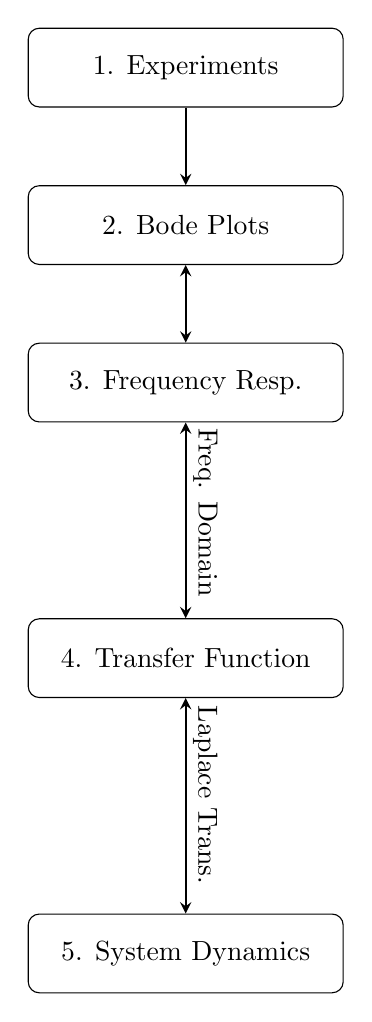
\begin{tikzpicture}[node distance = 2cm]
\node (start) [startstop] {1. Experiments};
\node (step1) [startstop,below of = start] {2. Bode Plots};
\node (step2) [startstop, below of = step1] {3. Frequency Resp.};
\node (step3) [startstop,below of  = step2, yshift = -1.5cm] {4. Transfer Function};
\node (step4) [startstop, below of = step3, yshift = -1.75cm] {5. System Dynamics};
\draw[arrow2](start)--(step1);
\draw[arrow1](step1)--(step2);
\draw[arrow1](step2)--(step3) node[midway,right, rotate = 270,xshift = -1.3cm, yshift = 0.25cm]{Freq. Domain};
\draw[arrow1](step3)--(step4) node[midway,right, rotate = 270,xshift = -1.4cm, yshift = 0.25cm]{Laplace Trans.};
\end{tikzpicture}
\captionof{figure}{Project Outline}
\label{Process}


&
\vspace{0pt}
The project itself is fairly straightforward. Teams of students will 
be given a simulated ``Black Box" system, and it will be your job to design a 
controller that will control the outputs of this system, given a set of performance 
specifications. Figure ~\ref{Process} gives a general outline for the 
steps you will be required to take in order to successfully do this. The techniques 
you will learn in these labs will be useful for your project. 
\begin{enumerate}
\item In lab~\ref{chap:freqresp} you will be conducting experiments on the DC motor by 
applying various voltages and measuring the difference between the desired input, and the 
actual output (in this case, the outputs will be angular position and angular velocity of the motor). 
These will give you the necessary information to construct what is called a Bode plot. 
\item A Bode plot is a graph of a systems frequency response. More specifically, several sinusoids 
of varying frequencies will be inputted into the system, then the magnitude and phase difference 
of the desired input vs the actual output will be measured, and plotted on a logarithmic scale. 
These plots are in the frequency domain, therefore they are plots of frequency ($\omega$) 
vs magnitude ($dB$), or frequency ($\omega$) vs phase difference ($rads$).
\end{enumerate}
\end{tabular}
\begin{enumerate}
	\setcounter{enumi}{2}
\item Once you have both Bode plots (magnitude and phase), it is then possible to determine 
your systems frequency response. The frequency response is in the form of a polynomial with various poles and zeros 
in the complex plane. The general shape of a Bode plot is dependent on the number of poles and zeros, 
and their location in the complex plane. Therefore, it is possible to determine the frequency response from 
your experimental bode plots. 
\item The transfer function of a system is what relates the inputs and outputs. If the dynamics of your system are unknown, 
then you have what is called a \emph{Black Box System}. When given a black box system, the transfer 
function is unknown, and you will want to determine an accurate model for it so that you can begin to control the 
system. To determine the transfer function from the frequency response, you must simply substitute the Laplace variable 
$s$ in place of $j\omega$.
\item The dynamics of a given system are typically given by some differential equation. See equation~\ref{eq:motor} 
for the governing equation of the DC motor you will be using in the labs. To find a transfer function for this system, you 
need to work in the \emph{Laplace} domain. This is done by creating  a variable $s=j\omega$, and taking the 
Laplace transform. You may want to review your notes from MTHE 237 on this topic. Once you have taken the 
Laplace transform, you can assess the open-loop stability of the system, and the frequency response. \\
Similarly, you can recover the governing equation of the system from the transfer function by simply taking 
the inverse Laplace transform. For your project, it is at this point that you will begin designing your controller. 
\end{enumerate}
Note that this intro may not be completely clear right away. You may find that as you work through the labs, and 
attend the weekly tutorials that the material will make more sense. This will also be a helpful reference guide 
throughout the project. 